%!TEX root = ../Thesis.tex
\chapter{Genetic markers of hub connectivity in the human brain}
\label{appendixC}
\fancyhead[R]{\textit{Appendix C:~Genetic markers of hub connectivity in the human brain}}

\section{Processing gene expression data}
\label{app:AppendixCh5_1}

Microarray gene expression and all the accompanying metadata were downloaded from the \url{http://human.brain-map.org/static/download}. The raw data consisted of \num{58692} probes quantifying the expression of \num{20737} genes in \num{3702} tissue samples in six neurotypical adult brains. The pre-processing procedures applied to the data are outlined below and the choices detailed in \mbox{\citep{Arnatkeviciute2019}}. Data used for the analyses can be found in the figshare repository: \url{https://figshare.com/s/441295fe494375aa0c13}.

\begin{enumerate}\addtocounter{enumii}{5}% This cannot be more than 25
      \item Probe-to-gene annotations were updated Re-Annotator software toolbox \citep{Arloth2015} resulting in the selection of \num{45821} probes corresponding to the total of \num{20232} genes.
      \item Tissue samples annotated to the brainstem and cerebellum were removed.
      \item Intensity based filtering was applied in order to exclude probes that do not exceed the background noise in more than 50\% of cortical and subcortical samples excluding \num{13844} probes corresponding to \num{4486} unique genes.
      \item If more than one probe was available for a gene, a representative probe was selected based on the correlation to RNA sequencing data \citep{Miller2014a} by applying several additional thresholding criteria:
      \begin{enumerate}
      \item genes that did not have the corresponding RNA-seq measures were removed;
      \item probes that demonstrated a low correlation to RNA-seq data (Spearman $\rho<0.2$) were removed;
	  \item a representative probe for a gene was selected based on the highest correlation to the RNA-seq data in the corresponding samples.
      \end{enumerate}
      \item Gene expression samples were assigned to the regions-of-interest by generating donor-specific grey matter parcellations and assigning samples located within $2$ mm of the parcellation voxels. To increase the assignment accuracy, samples were first divided into four separate groups based on their location: hemisphere (left/right) and structure assignment (cortex/subcortex), so samples listed as coming from the left cortical hemisphere as per AHBA ontology are only mapped to left cortical voxels of the parcellation. Applying $2$ mm distance threshold almost 90\% of all cortical and subcortical samples were assigned to a non-zero voxel of the parcellation.
      \item Samples assigned to the subcortical regions as well as samples assigned to the right hemisphere were removed.
      \item To account for inter-individual differences in gene expression between the donor brains, gene expression measures within a given brain (left cortical samples) were normalised by applying a scaled robust sigmoid normalisation \citep{Arnatkeviciute2019} in two separate steps:
      \begin{enumerate}
      \item For every sample across all genes to quantify the relative expression of every gene within each sample;
      \item For every gene across all samples to evaluate the relative expression of each gene across regions.
      \end{enumerate}
      \item The resulting normalised expression measures assigned to the same region in the parcellation were averaged and aggregated into a region by gene matrix consisting of expression measures for \num{10027} genes over 180 and 250 cortical regions respectively.
      \item Distances between those regions were estimated on the cortical surface (pial) using the annotation files for each parcellation, the spherical and the fsaverage representation of the cortical surface. First, all the vertices that correspond to a particular region in the spherical representation were identified and their centroid coordinates were calculated. Then the centroid coordinates were mapped to the fsaverage cortical surface and the distances between each pair of regions were calculated using the toolbox \texttt{fast\_marching\_toolbox} in MATLAB.
\end{enumerate}

\newpage
\section{Robustness to data processing decisions}
\label{app:AppendixCh5_2}

In this section we show robustness checks for data processing decisions. To evaluate how sensitive our findings are to the parcellation and connection density choices, here we present a set of the main findings using two different parcellations containing i) 360 functionally defined (f360) and ii) 500 randomly defined (r500) regions at different connectome densities. If not stated otherwise, the top row (panels A-C) contains results replicated using f360 parcellation and the bottom row (panels D-F) -- r500 parcellation. In all cases connectomes maintain the topological (Figure \ref{fig:Ch5SFig1}) and weighted (Figure \ref{fig:Ch5SFig2}) rich-club organisation with a slightly increasing consistency of the effect for the topological rich-club organisation at higher connectome densities (compare Figure \ref{fig:Ch5SFig1} A and C; D and F).

\begin{figure}[h!]
\begin{center}
\includegraphics[width=1\textwidth]{Chapter5/SFigure1.pdf}% This is a *.eps file
\end{center}
\caption{\textbf{Topological rich-club.}
Topological rich-club results reproduced using: top row -- 360 region parcellation at $15\%$ (A), $20\%$ (B), $25\%$ (C) connectome density; bottom row -- 500 region parcellation at $10\%$ (D), $15\%$ (E), $20\%$ (F) connectome density. In each plot top: The degree distribution of the group-level connectome. Bottom: Normalised topological rich-club coefficient ($\Phi_{norm}$); $\Phi_{norm}>1$ indicates that hubs are more densely interconnected than expected by chance; circles indicate values that are significantly higher than an ensemble of 1000 degree-matched null networks ($p<0.05$).}
\label{fig:Ch5SFig1}
\end{figure}

\begin{figure}[h!]
\begin{center}
\includegraphics[width=1\textwidth]{Chapter5/SFigure2.pdf}% This is a *.eps file
\end{center}
\caption{\textbf{Weighted rich-club.}
Weighted rich-club results reproduced using: top row -- 360 region parcellation at $15\%$ (A), $20\%$ (B), $25\%$ (C) connectome density; bottom row -- 500 region parcellation at $10\%$ (D), $15\%$ (E), $20\%$ (F) connectome density. In each plot top: The degree distribution of the group-level connectome. Bottom: Normalised weighted rich-club coefficient ($\Phi_{norm}$); $\Phi_{norm}>1$ indicates that connections between hubs are stronger than expected by chance; circles indicate values that are significantly higher than an ensemble of 1000 null networks ($p<0.05$) where the connections weights were randomised while preserving the topology. }
\label{fig:Ch5SFig2}
\end{figure}

\clearpage
Heritability estimates remain significantly increased for rich links in both f360 and r500 parcellations at all densities (Figure \ref{fig:Ch5SFig3}). Overall heritability estimates within the lower density connectomes were slightly higher compared to the denser ones (the dotted line shifts down along the columns). Connectomes defined based on the r500 parcellation demonstrate marginally lower heritability that might be related to the lower connectome density ($15-25\%$ \textit{vs} $10-20\%$). A little higher heritability for the rich links with a more consistent increase at the highest degrees were obtained using a f360 parcellation likely due to a slightly higher number of nodes at the very end of the degree distribution.

\begin{figure}[h!]
\begin{center}
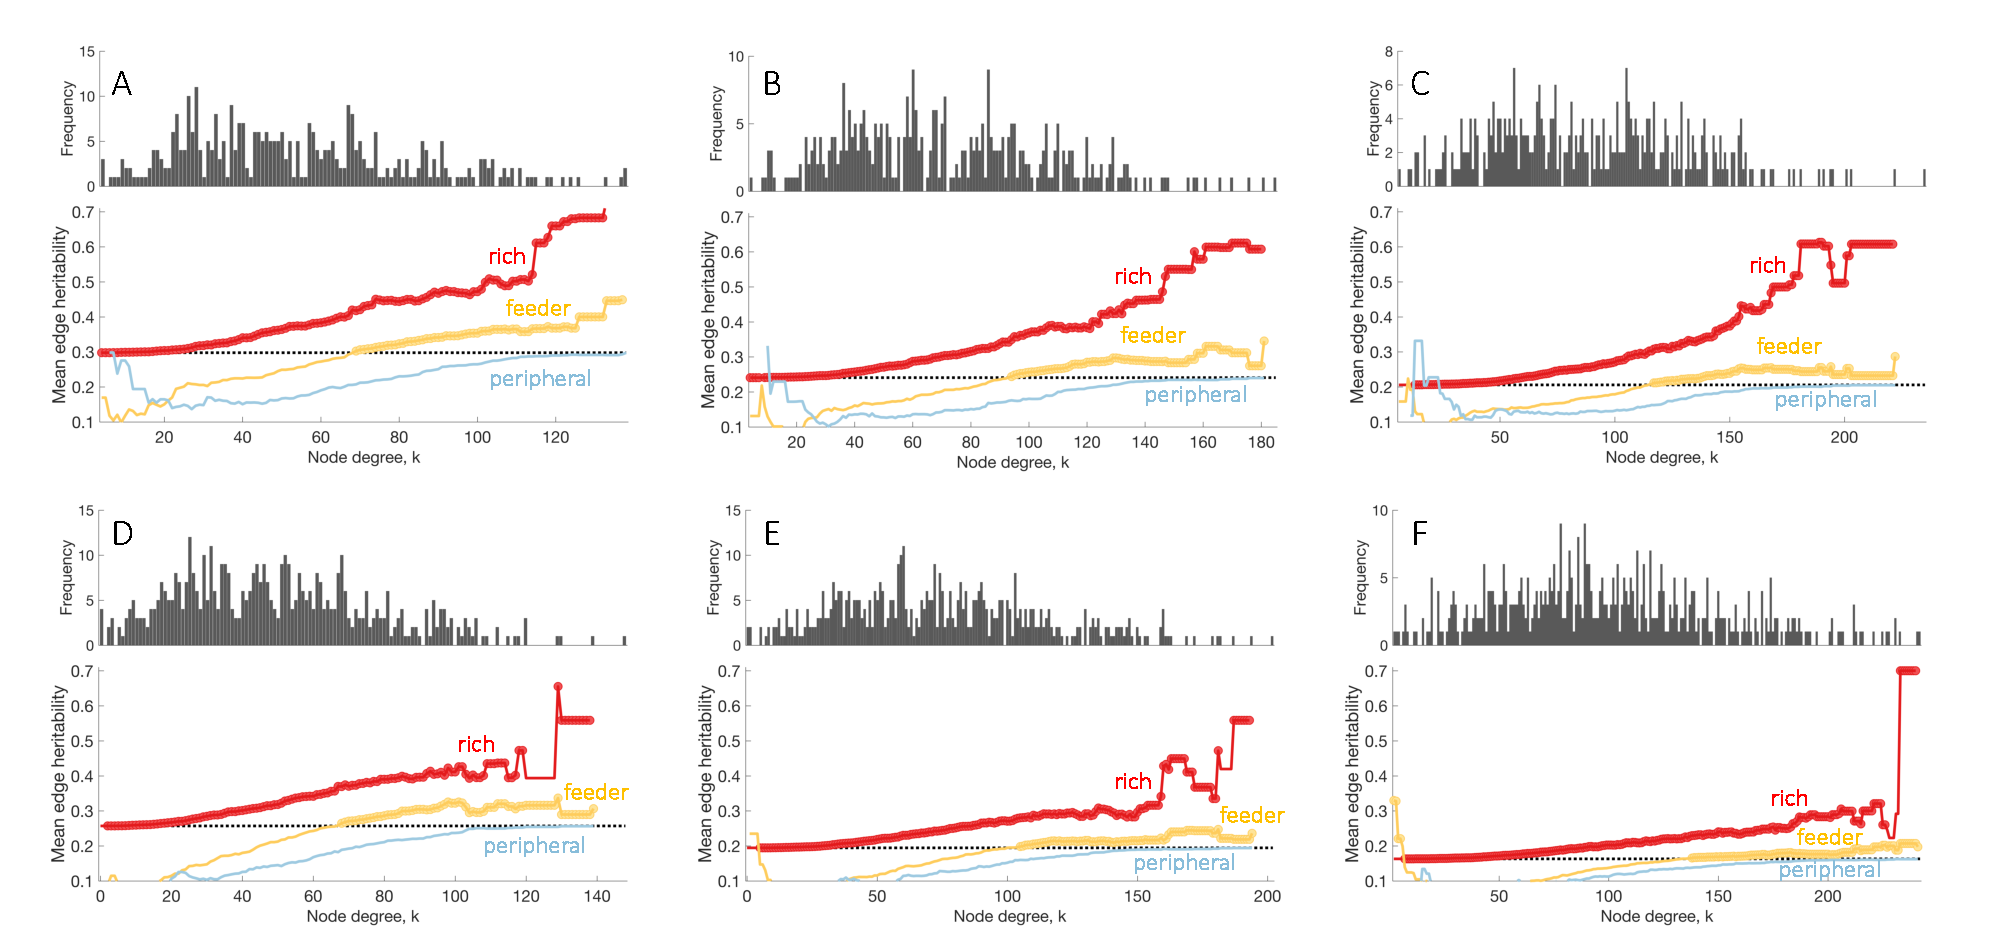
\includegraphics[width=1\textwidth]{Chapter5/SFigure3.pdf}% This is a *.eps file
\end{center}
\caption{\textbf{Heritability.}
Mean edge heritability results reproduced using: top row -- 360 region parcellation at $15\%$ (A), $20\%$ (B), $25\%$ (C) connectome density; bottom row -- 500 region parcellation at $10\%$ (D), $15\%$ (E), $20\%$ (F) connectome density. In each plot top: The degree distribution of the group-level connectome. Bottom: Mean edge heritability for `rich' (hub -- hub), `feeder' (hub -- nonhub), `peripheral' (nonhub -- nonhub) connections as a function of degree threshold, \textit{k} used to define hubs. The mean heritability across all network links shown as a dotted black line. Circles indicate a statistically significant increase in heritability in a given link type compared to the rest of the network (one-sided Welch's $t$-test, $p < 0.05$).}
\label{fig:Ch5SFig3}
\end{figure}

\clearpage
Correlated gene expression remains significantly increased for rich links in both parcellations across a range of degree thresholds (Figure \ref{fig:Ch5SFig4}). Within the functionally defined parcellation, the increase in CGE is more pronounced at the lower connectome densities which might be related to the potentially increased number of false positive connections at higher densities. Comparable results for rich links are evident within the r500 parcellation with feeder links demonstrating a more significant increase in CGE compared to only a marginal effect in f360 parcellation.

\begin{figure}[h!]
\begin{center}
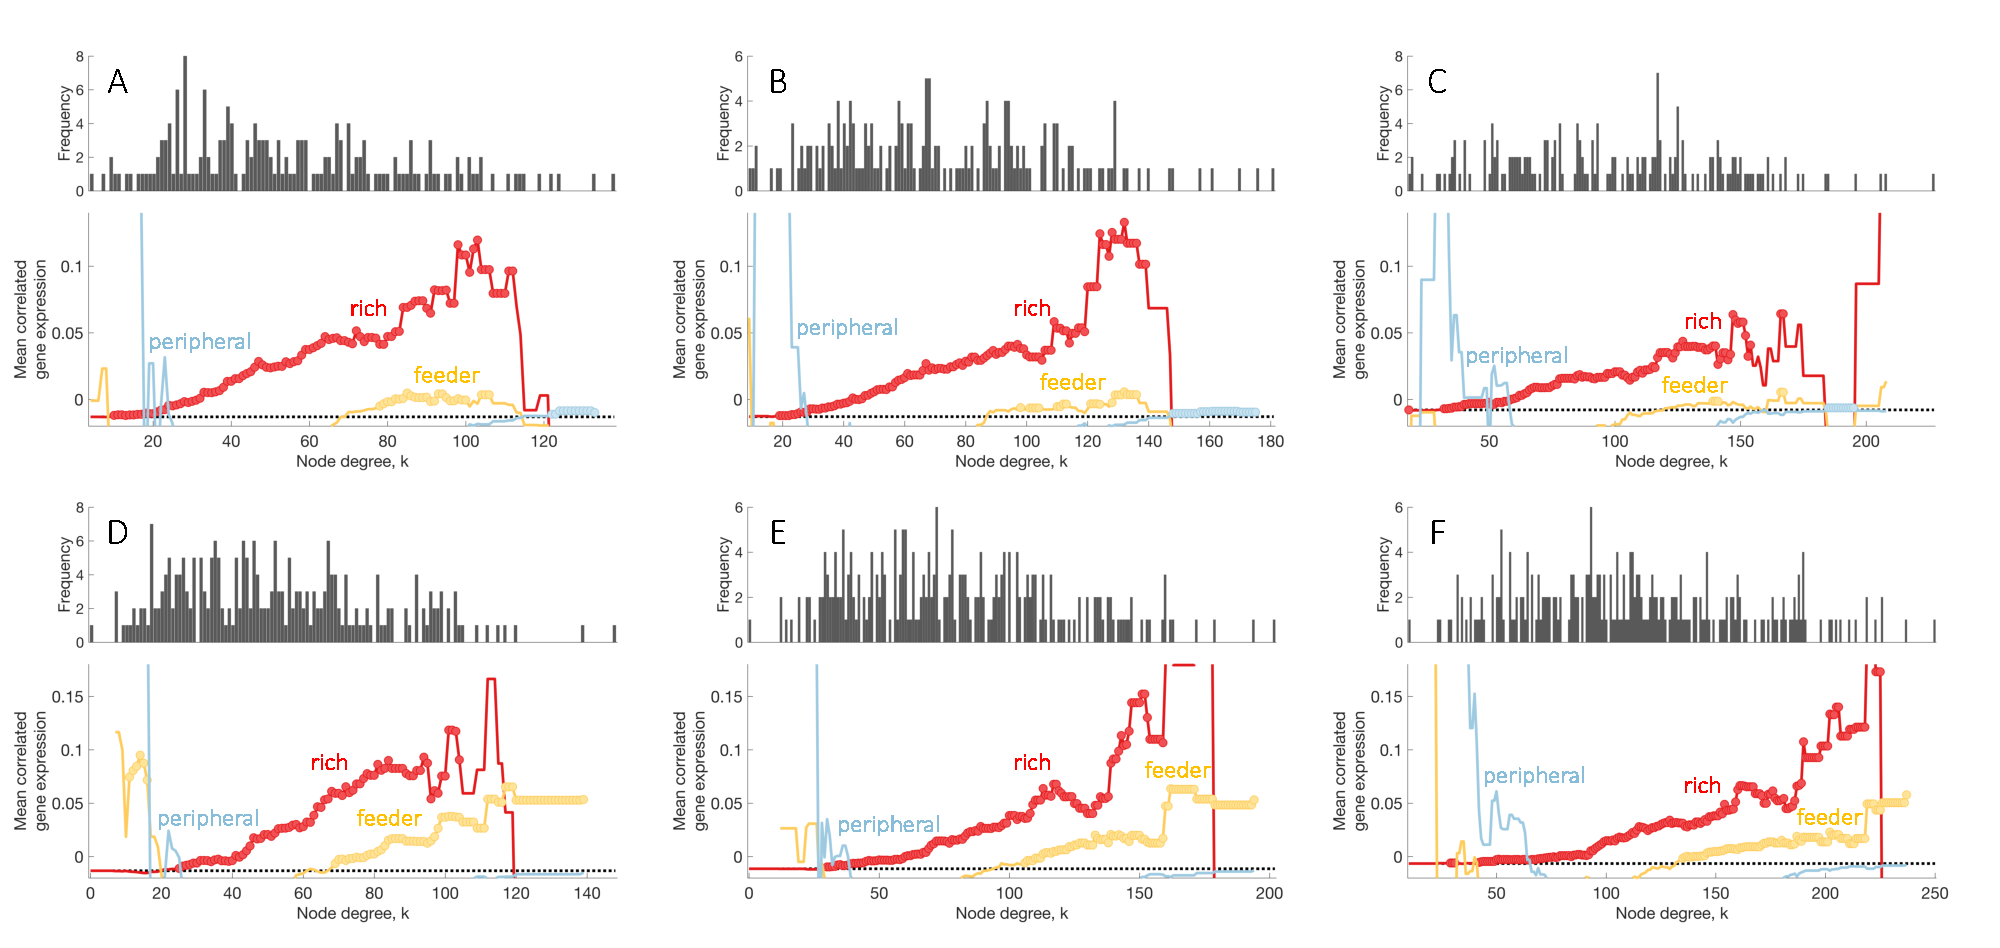
\includegraphics[width=1\textwidth]{Chapter5/SFigure4.pdf}% This is a *.eps file
\end{center}
\caption{\textbf{Transcriptional coupling.}
Mean correlated gene expression results reproduced using: top row -- 360 region parcellation at $15\%$ (A), $20\%$ (B), $25\%$ (C) connectome density; bottom row -- 500 region parcellation at $10\%$ (D), $15\%$ (E), $20\%$ (F) connectome density. In each plot top: The degree distribution of the group-level connectome. Bottom: Mean correlated gene expression for `rich' (hub -- hub), `feeder' (hub -- nonhub), `peripheral' (nonhub -- nonhub) connections as a function of degree threshold, \textit{k} used to define hubs. The mean correlated gene expression across all network links shown as a dotted black line. Circles indicate a statistically significant increase in correlated gene expression in a given link type compared to the rest of the network (one-sided Welch's $t$-test, $p < 0.05$).}
\label{fig:Ch5SFig4}
\end{figure}

\clearpage
Comparable decrease in the association between the connection weight and polygenic score for bipolar disorder (Figure \ref{fig:Ch5SFig5}), ASD (Figure \ref{fig:Ch5SFig6}) and major depression (Figure \ref{fig:Ch5SFig9}) were obtained in both parcellations and across connection densities. In those cases connectomes based on the r500 parcellation demonstrated a decrease over a wider range of values. The associations for schizophrenia (Figure \ref{fig:Ch5SFig7}) and ADHD (Figure \ref{fig:Ch5SFig8}) remain consistent across all densities of the f360 parcellation, however are not reproduced using r500 parcellation. The relationship between the connection weight and polygenic scores for IQ (Figure \ref{fig:Ch5SFig10}) were consistent across a range of connectome densities within the f360 parcellation whereas demonstrating only a marginal increase for rich links in r500 connectomes. Considering that the parcellations differ in region definition (functional \textit{vs} random), resolution and region size it is difficult to disentangle the contribution of each factor.

\begin{figure}[h!]
\begin{center}
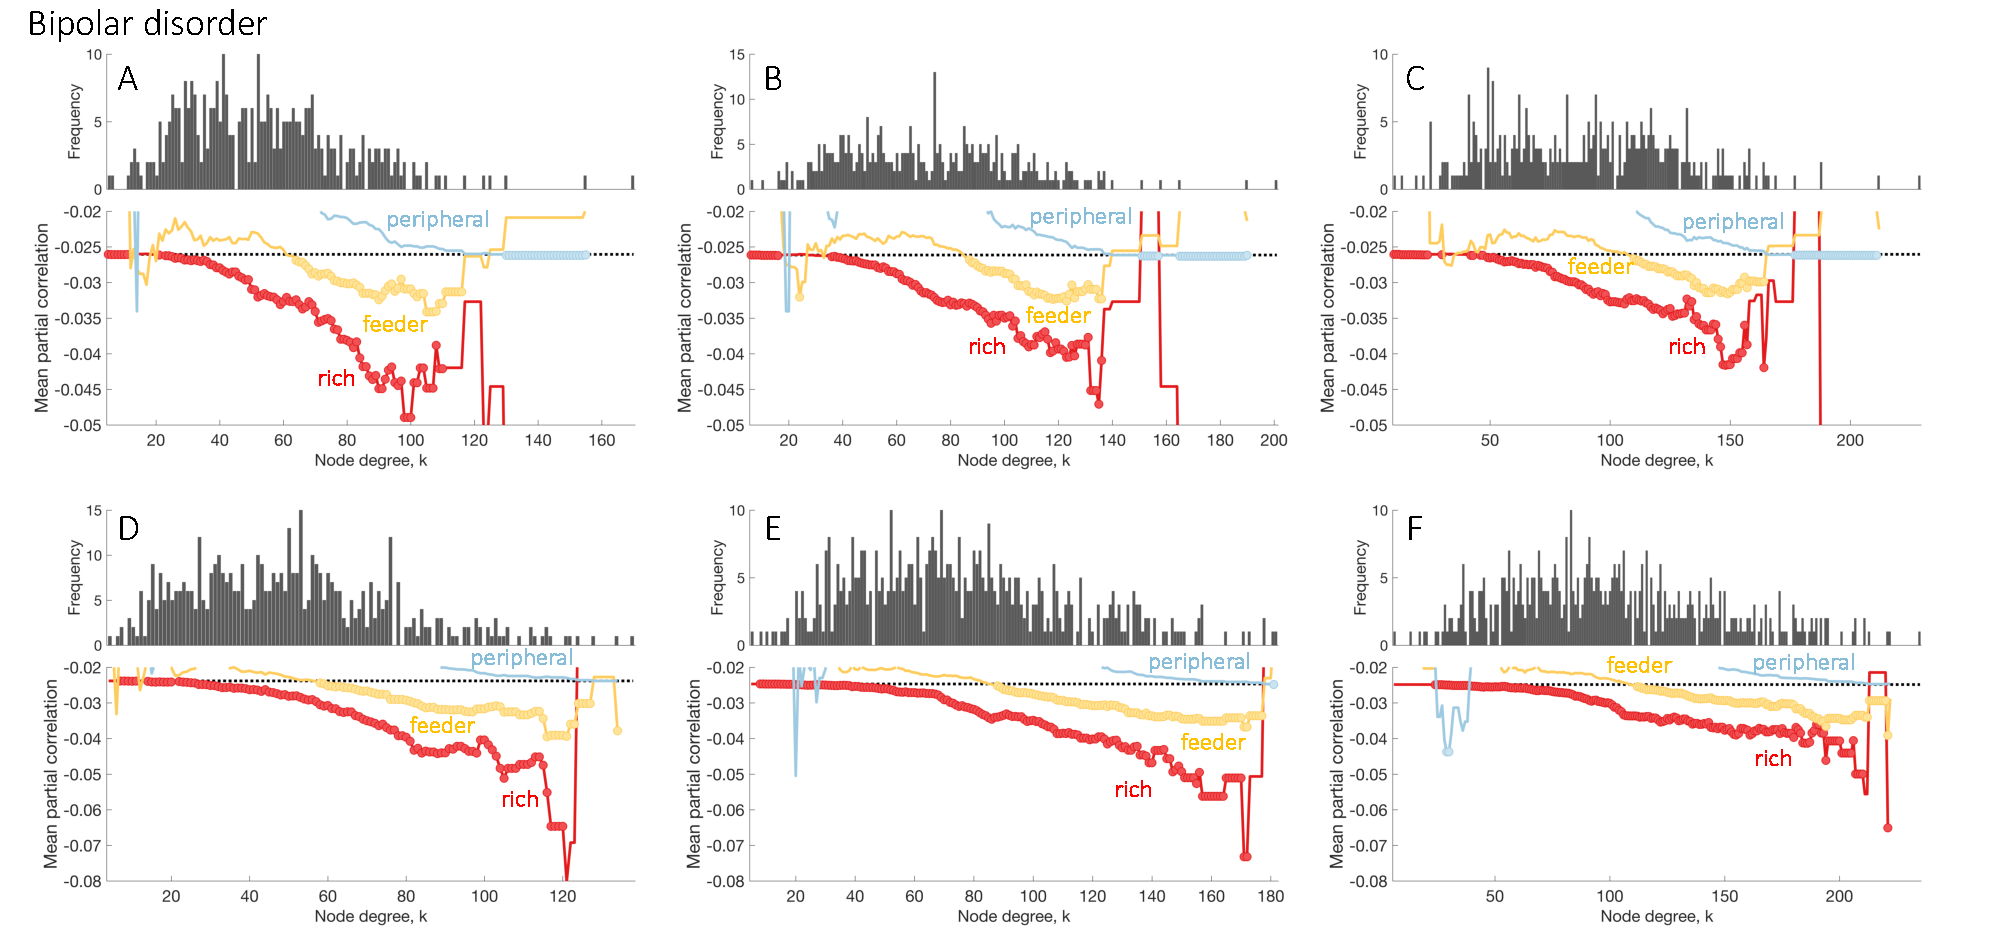
\includegraphics[width=1\textwidth]{Chapter5/SFigure5.pdf}% This is a *.eps file
\end{center}
\caption{\textbf{PGS correlation: bipolar disorder.}
The bipolar disorder polygenic score results reproduced using: top row -- 360 region parcellation at $15\%$ (A), $20\%$ (B), $25\%$ (C) connectome density; bottom row -- 500 region parcellation at $10\%$ (D), $15\%$ (E), $20\%$ (F) connectome density. In each plot top: The degree distribution of the group-level connectome. Bottom: Mean partial correlation (Spearman) coefficient between the connection weight and polygenic scores for bipolar disorder for each connection type as a function of \textit{k}. The mean partial correlation across all network links is shown as a dotted black line; Circles indicate a statistically significant decrease in correlation coefficient in a given link type relative to the rest of the network (one-sided Welch's $t$-test, $p < 0.05$).}
\label{fig:Ch5SFig5}
\end{figure}

\begin{figure}[h!]
\begin{center}
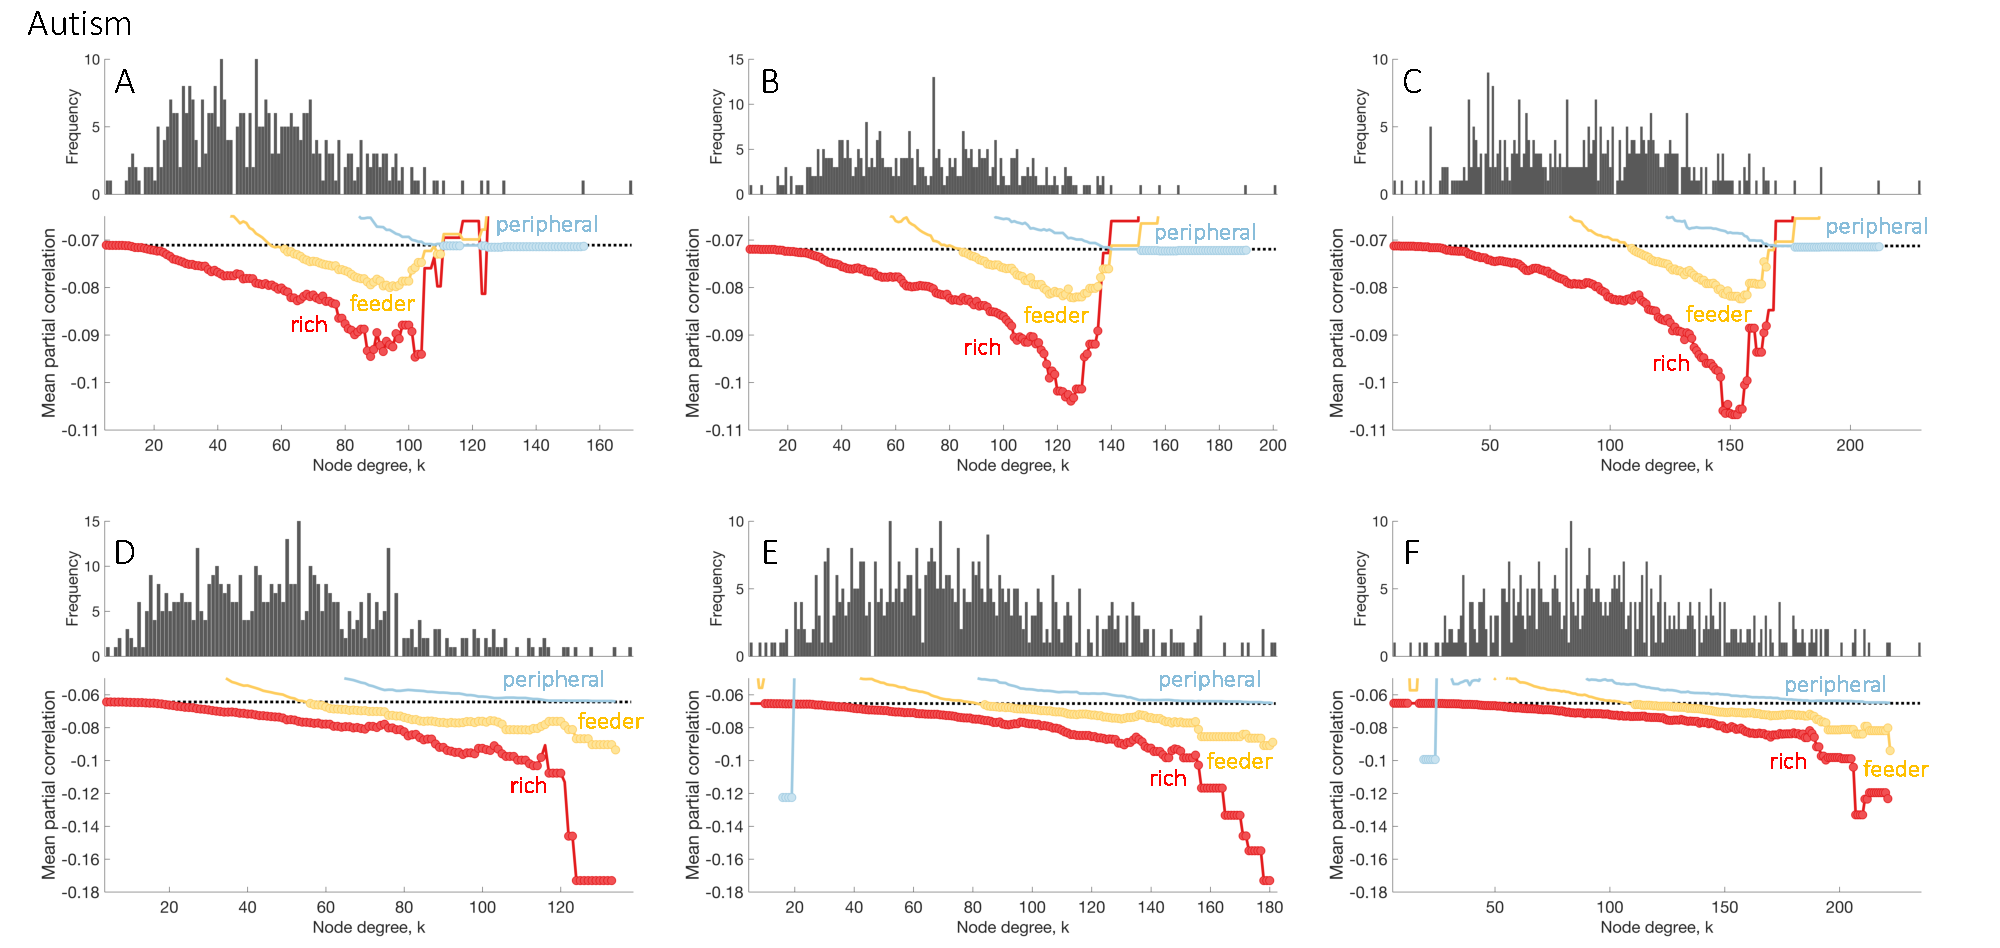
\includegraphics[width=1\textwidth]{Chapter5/SFigure6.pdf}% This is a *.eps file
\end{center}
\caption{\textbf{PGS correlation: ASD.}
The autism spectrum disorder polygenic score results reproduced using: top row -- 360 region parcellation at $15\%$ (A), $20\%$ (B), $25\%$ (C) connectome density; bottom row -- 500 region parcellation at $10\%$ (D), $15\%$ (E), $20\%$ (F) connectome density. In each plot top: The degree distribution of the group-level connectome. Bottom: Mean partial correlation (Spearman) coefficient between the connection weight and polygenic scores for autism spectrum disorder for each connection type as a function of \textit{k}. The mean partial correlation across all network links is shown as a dotted black line; Circles indicate a statistically significant decrease in correlation coefficient in a given link type relative to the rest of the network (one-sided Welch's $t$-test, $p < 0.05$).}
\label{fig:Ch5SFig6}
\end{figure}

\begin{figure}[h!]
\begin{center}
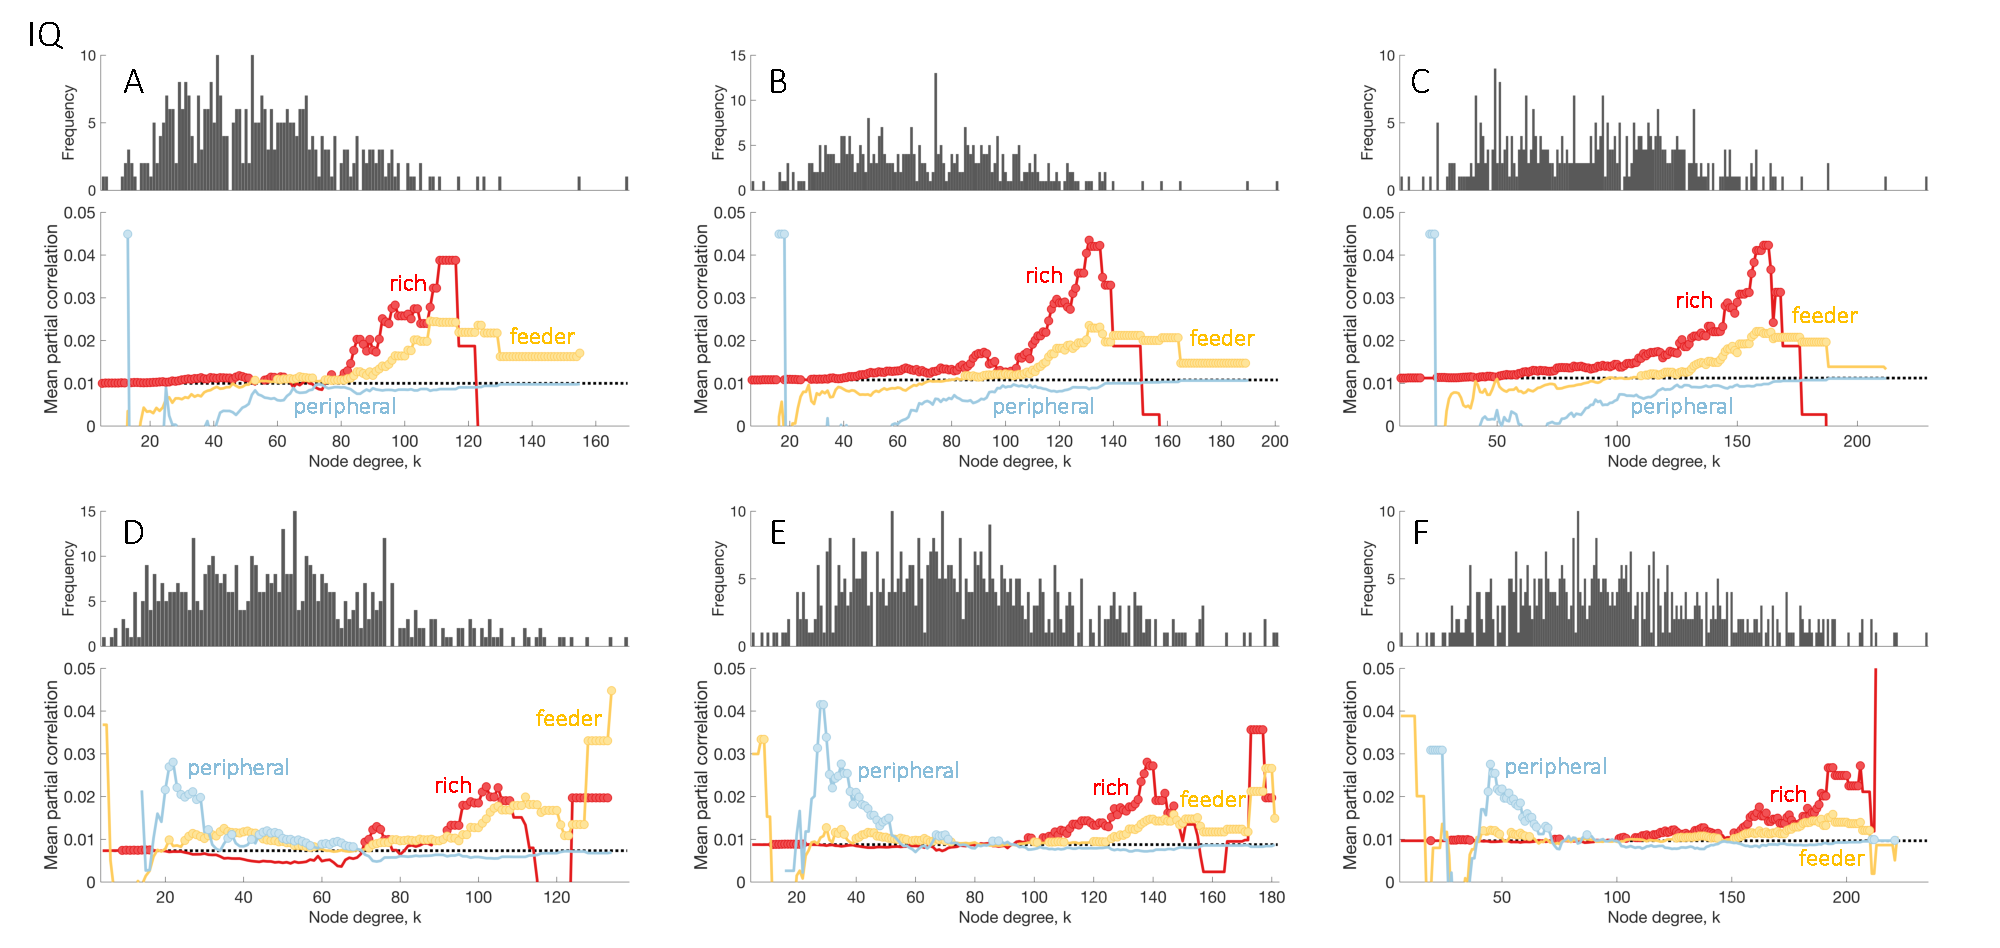
\includegraphics[width=1\textwidth]{Chapter5/SFigure9.pdf}% This is a *.eps file
\end{center}
\caption{\textbf{PGS correlation: major depression.}
The major depression polygenic score results reproduced using: top row --  360 region parcellation at $15\%$ (A), $20\%$ (B), $25\%$ (C) connectome density; bottom row -- 500 region parcellation at $10\%$ (D), $15\%$ (E), $20\%$ (F) connectome density. In each plot top: The degree distribution of the group-level connectome. Bottom: Mean partial correlation (Spearman) coefficient between the connection weight and polygenic scores for major depression for each connection type as a function of \textit{k}. The mean partial correlation across all network links is shown as a dotted black line; Circles indicate a statistically significant decrease in correlation coefficient in a given link type relative to the rest of the network (one-sided Welch's $t$-test, $p < 0.05$).}
\label{fig:Ch5SFig9}
\end{figure}

\begin{figure}[h!]
\begin{center}
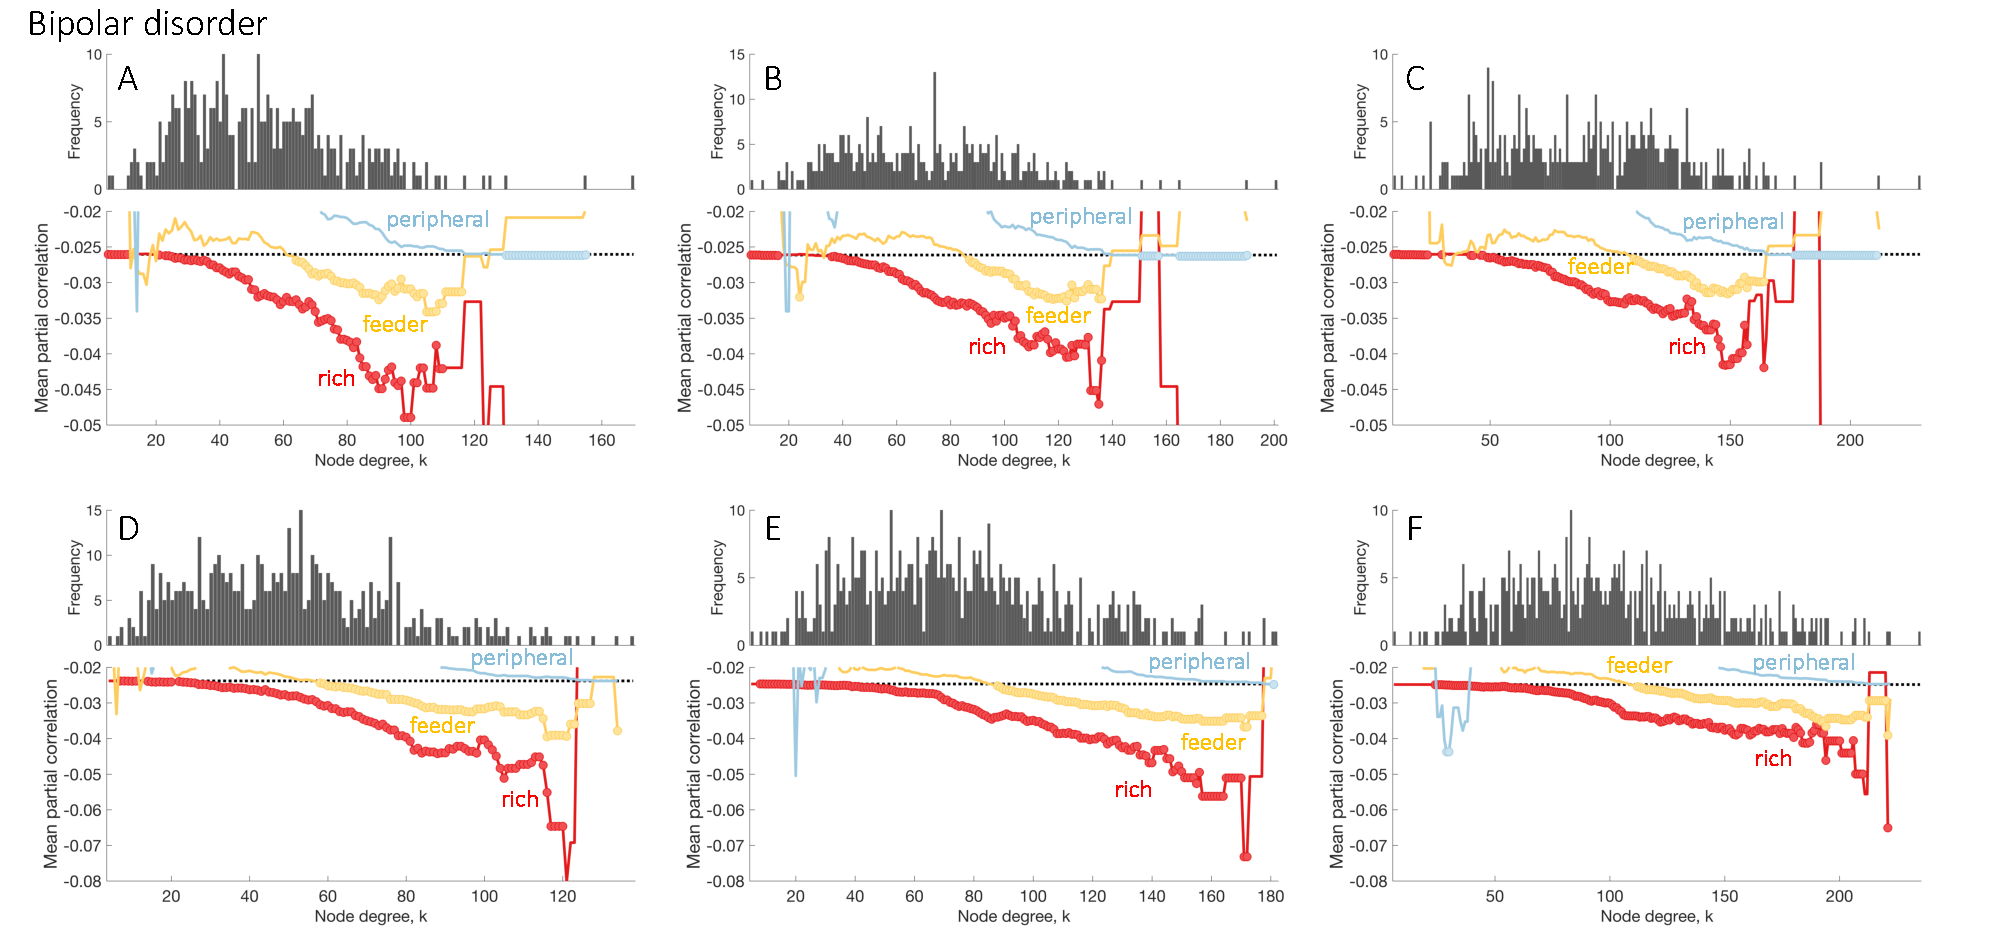
\includegraphics[width=1\textwidth]{Chapter5/SFigure7.pdf}% This is a *.eps file
\end{center}
\caption{\textbf{PGS correlation: schizophrenia.}
The schizophrenia polygenic score results reproduced using: top row -- 360 region parcellation at $15\%$ (A), $20\%$ (B), $25\%$ (C) connectome density; bottom row -- 500 region parcellation at $10\%$ (D), $15\%$ (E), $20\%$ (F) connectome density. In each plot top: The degree distribution of the group-level connectome. Bottom: Mean partial correlation (Spearman) coefficient between the connection weight and polygenic scores for schizophrenia for each connection type as a function of \textit{k}. The mean partial correlation across all network links is shown as a dotted black line; Circles indicate a statistically significant decrease in correlation coefficient in a given link type relative to the rest of the network (one-sided Welch's $t$-test, $p < 0.05$).}
\label{fig:Ch5SFig7}
\end{figure}

\begin{figure}[h!]
\begin{center}
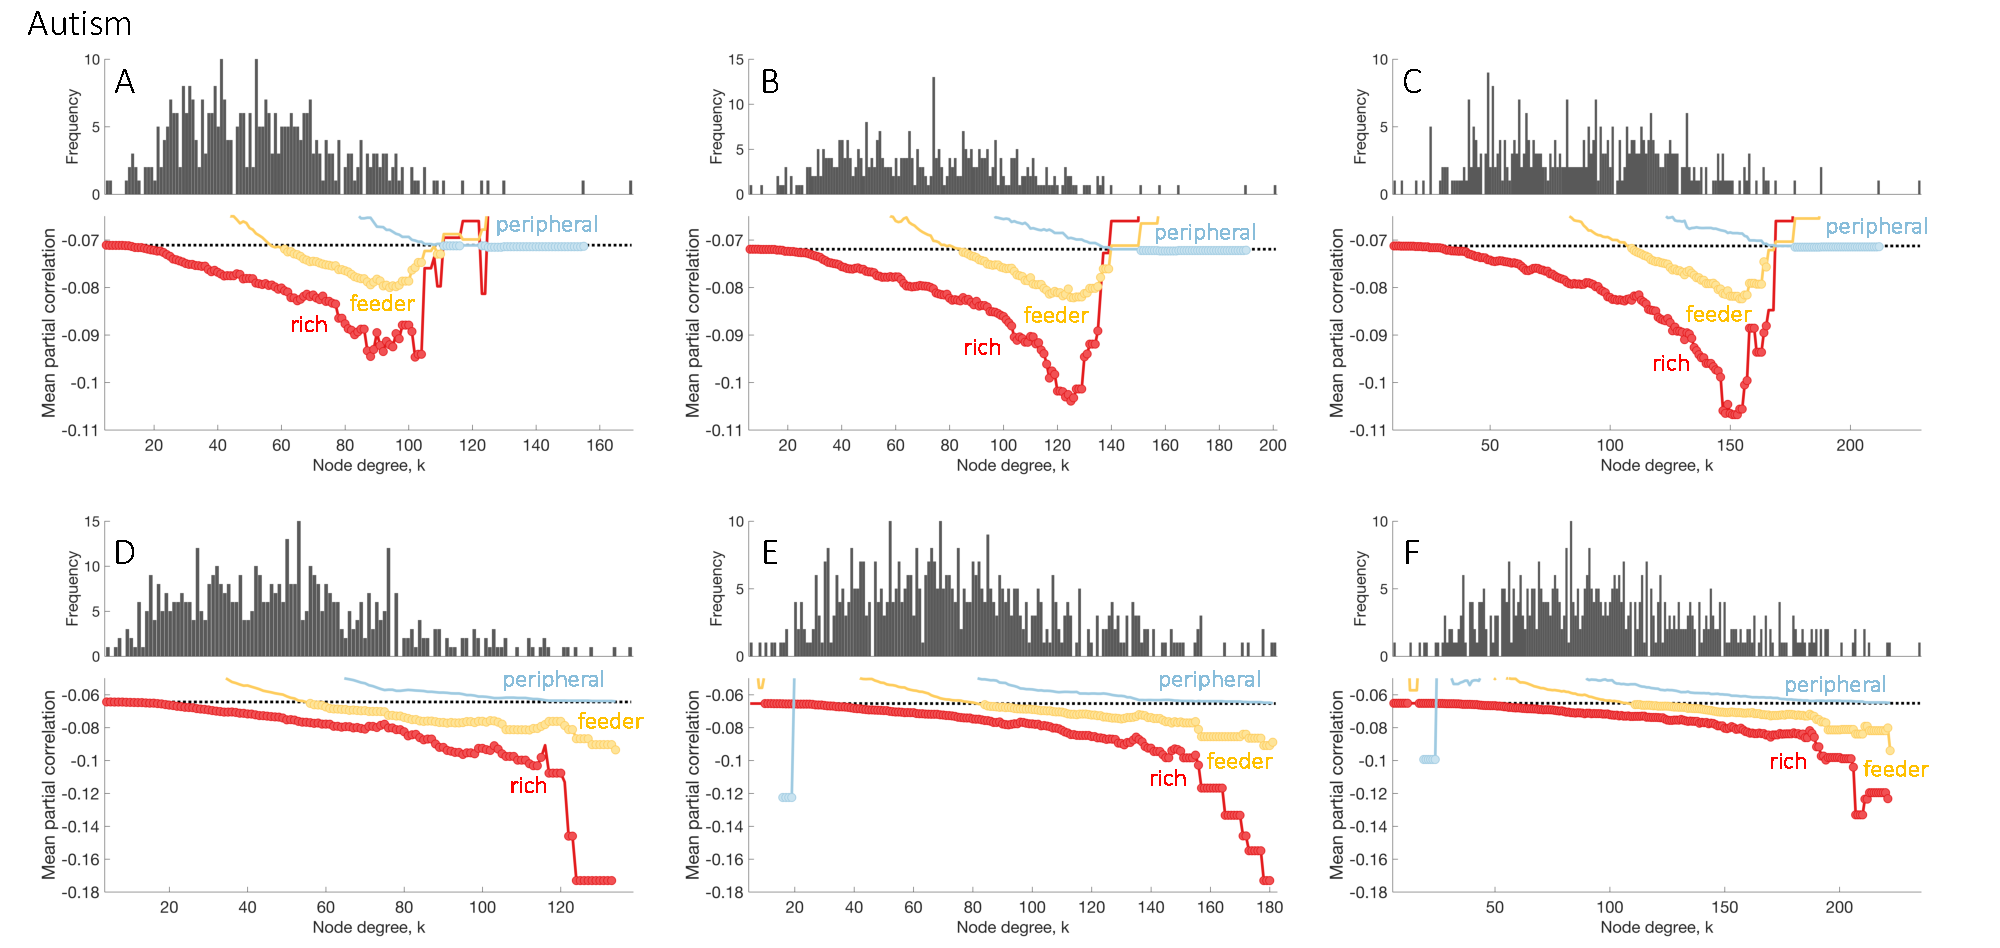
\includegraphics[width=1\textwidth]{Chapter5/SFigure8.pdf}% This is a *.eps file
\end{center}
\caption{\textbf{PGS correlation: ADHD.}
The ADHD polygenic score results reproduced using: top row -- 360 region parcellation at $15\%$ (A), $20\%$ (B), $25\%$ (C) connectome density; bottom row -- 500 region parcellation at $10\%$ (D), $15\%$ (E), $20\%$ (F) connectome density. In each plot top: The degree distribution of the group-level connectome. Bottom: Mean partial correlation (Spearman) coefficient between the connection weight and polygenic scores for ADHD for each connection type as a function of \textit{k}. The mean partial correlation across all network links is shown as a dotted black line; Circles indicate a statistically significant decrease in correlation coefficient in a given link type relative to the rest of the network (one-sided Welch's $t$-test, $p < 0.05$).}
\label{fig:Ch5SFig8}
\end{figure}

\begin{figure}[h!]
\begin{center}
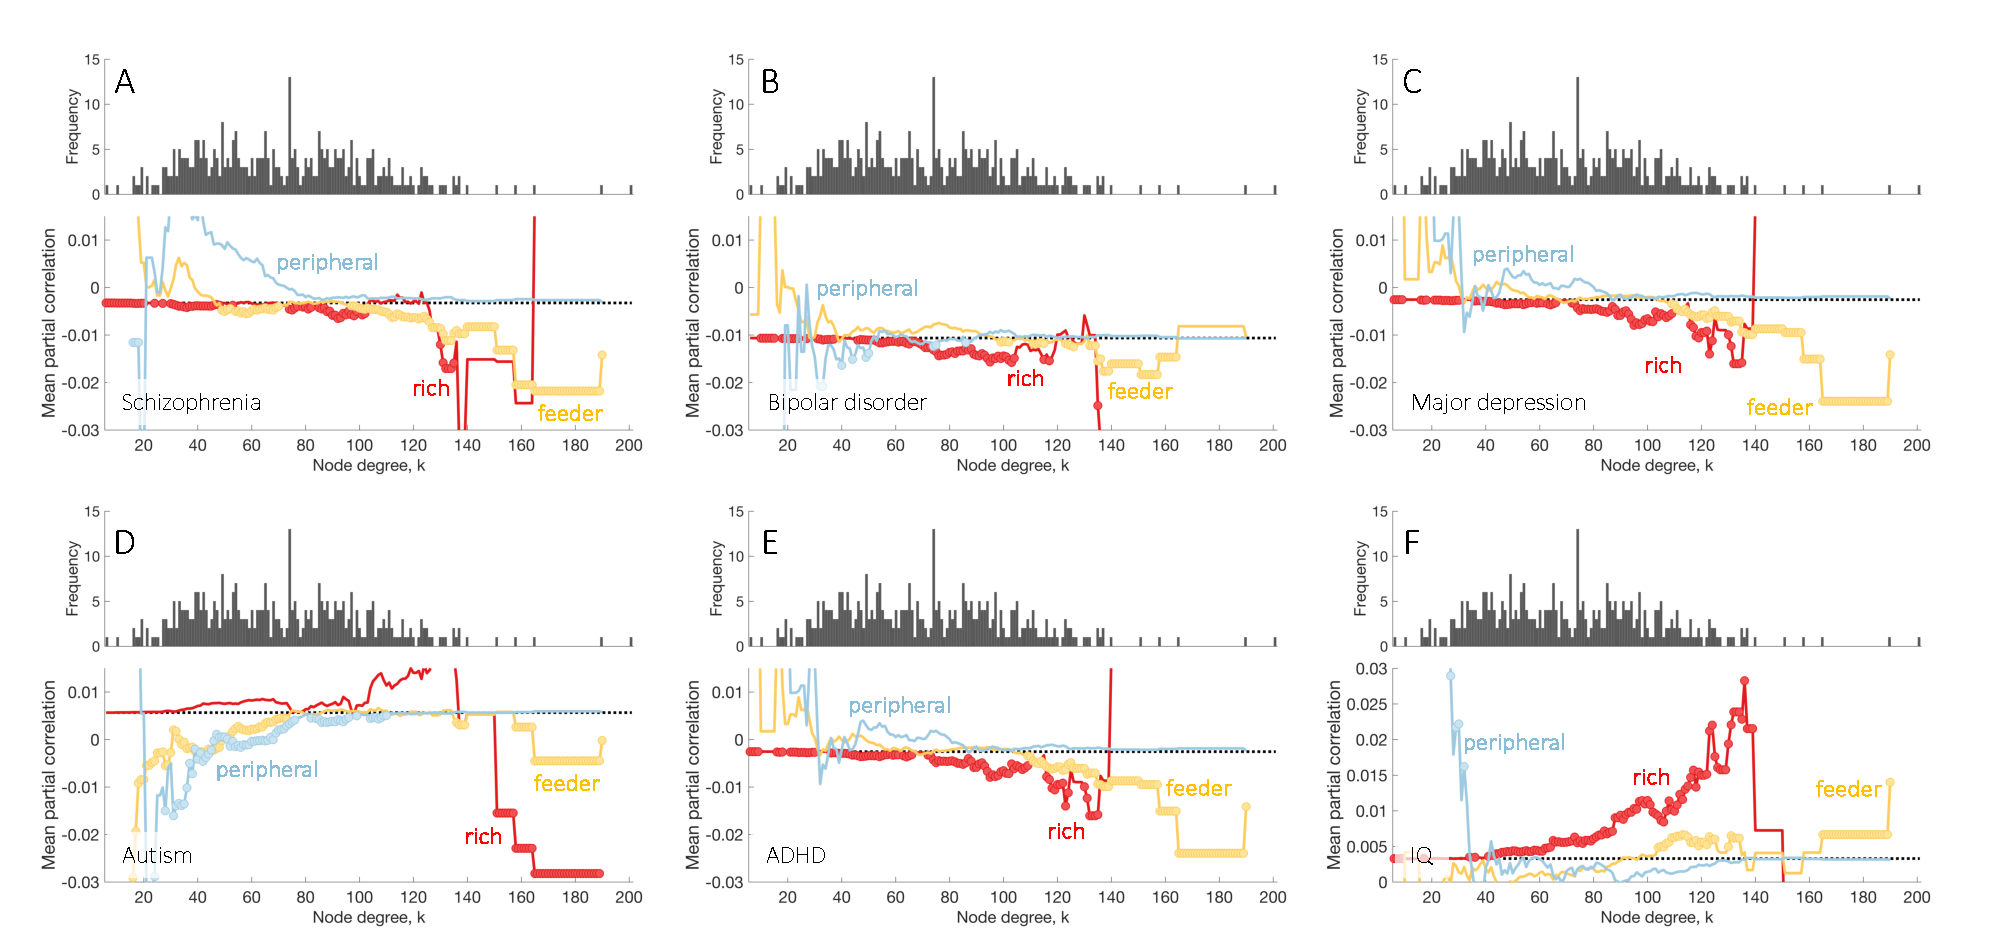
\includegraphics[width=1\textwidth]{Chapter5/SFigure10.pdf}% This is a *.eps file
\end{center}
\caption{\textbf{PGS correlation: IQ.}
The IQ polygenic score results reproduced using: top row -- 360 region parcellation at $15\%$ (A), $20\%$ (B), $25\%$ (C) connectome density; bottom row -- 500 region parcellation at $10\%$ (D), $15\%$ (E), $20\%$ (F) connectome density. In each plot top: The degree distribution of the group-level connectome. Bottom: Mean partial correlation (Spearman) coefficient between the connection weight and polygenic scores for IQ for each connection type as a function of \textit{k}. The mean partial correlation across all network links is shown as a dotted black line; Circles indicate a statistically significant increase in correlation coefficient in a given link type relative to the rest of the network (one-sided Welch's $t$-test, $p < 0.05$).}
\label{fig:Ch5SFig10}
\end{figure}


\clearpage
In the following section the main heritability and PGS correlation analyses are reproduced using streamline count (SC) weighted connectomes. Heritability for rich links increases as a function of degree (Figure \ref{fig:Ch5SFig11}) resembling the trend observed in the fractional anisotropy-based connectomes. Overall heritability estimates are lower with the maximum values for rich links reaching around $0.3$ at the highest degree thresholds compared to $0.7$ in the cases where heritability was estimated based on FA weights. The observed trends in polygenic score correlation analyses are much weaker compared to the FA-based connectomes (Figure \ref{fig:Ch5SFig12}). Whereas in most cases the directionality of the effect is similar with some instances demonstrating comparable trends (Figure \ref{fig:Ch5SFig11}C,F), it is not possible to make any definitive statements from such results. One potential explanation regarding the lower heritability estimates and the limited reproducibility for the polygenic score analyses using streamline count to define connection weights might be related to the non-biological nature of the measure. Within the context of probabilistic tractography SC can be regarded as the relative measure of connection probability, however the raw values lack a direct biological interpretation. Moreover, SC-based weights extend over several orders of magnitude consequently complicating the outlier removal procedure that is important in both heritability and polygenic score correlation analyses.

\begin{figure}[h!]
\begin{center}
\includegraphics[width=0.8\textwidth]{Chapter5/SFigure11.pdf}% This is a *.eps file
\end{center}
\caption{\textbf{Heritability: SC.}
Top: The degree distribution of the representative group-level connectome. Bottom: Mean edge heritability for `rich' (hub -- hub), `feeder' (hub -- nonhub), `peripheral' (nonhub -- nonhub) connections as a function of degree threshold, \textit{k} used to define hubs. The mean heritability across all network links shown as a dotted black line. Circles indicate a statistically significant increase in heritability in a given link type compared to the rest of the network (one-sided Welch's $t$-test, $p < 0.05$). }
\label{fig:Ch5SFig11}
\end{figure}

\begin{figure}[h!]
\begin{center}
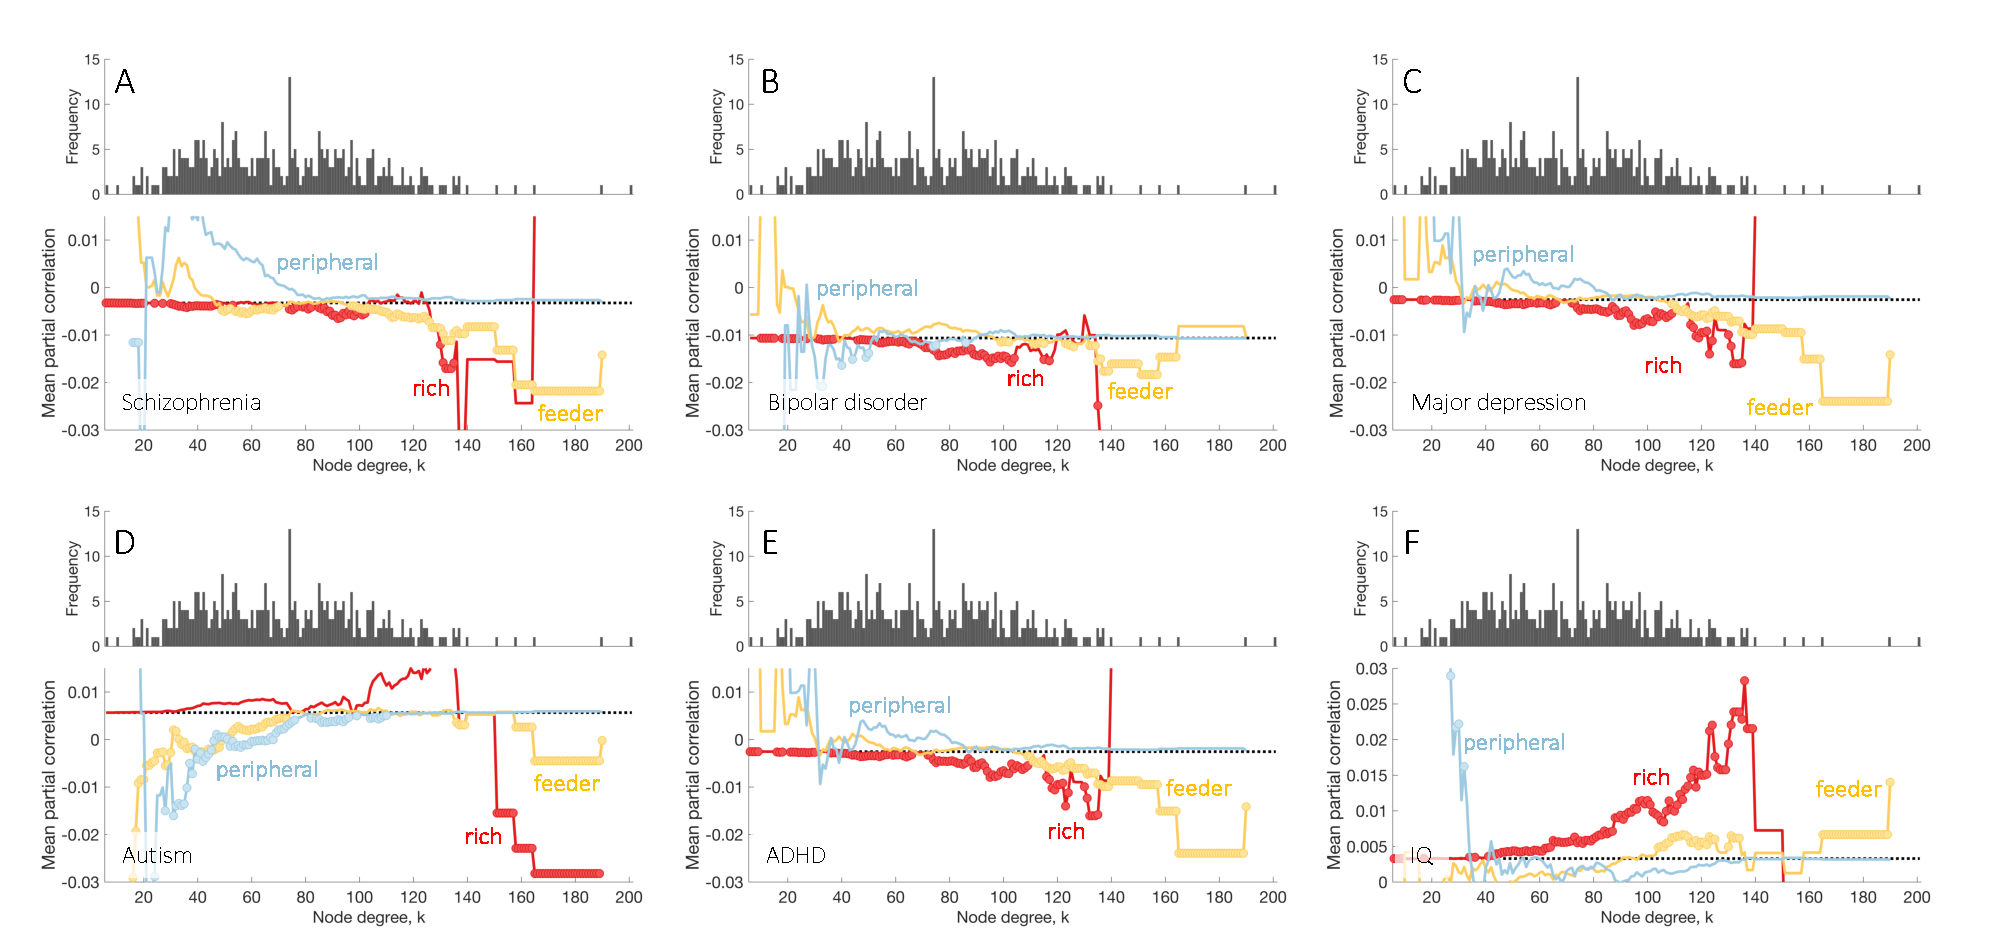
\includegraphics[width=1\textwidth]{Chapter5/SFigure12.pdf}% This is a *.eps file
\end{center}
\caption{\textbf{PGS correlation: SC.}
The connection weigh and polygenic score correlation analysis reproduced based on the streamline count weighted connectome using 360 region parcellation at $20\%$ density for a range of psychiatric disorder and IQ polygenic scores: A) schizophrenia; B) bipolar disorder; C) major depression; D) ASD; E) ADHD; F) IQ. Each plot: top: The degree distribution of the group-level connectome. Bottom: Mean partial correlation (Spearman) coefficient between the connection weight and polygenic scores for each connection type as a function of \textit{k}. The mean partial correlation across all network links is shown as a dotted black line; Circles indicate a statistically significant decrease (A-E) and increase (F) in correlation coefficient in a given link type relative to the rest of the network (one-sided Welch's $t$-test, $p < 0.05$). }
\label{fig:Ch5SFig12}
\end{figure}

\clearpage
\section{Gene enrichment results and rich-club organisation}
\label{app:AppendixCh5_3}

\begin{figure}[h!]
\begin{center}
\includegraphics[width=0.85\textwidth]{Chapter5/SFigure13.pdf}% This is a *.eps file
\end{center}
\caption{\textbf{Rich-club organisation of the group representative connectome derived from the Monash Cohort.} Top: the degree distribution of the connectome A) Normalised topological rich-club coefficient ($\Phi_\mathrm{{norm}}$); $\Phi_\mathrm{{norm}}>1$ indicates that hubs are more densely interconnected than expected by chance; red circles indicate values that are significantly higher than an ensemble of 1000 degree-matched null networks ($p<0.05$). B) Normalised weighted rich-club coefficient ($\Phi_\mathrm{{norm}}$); $\Phi_\mathrm{{norm}}>1$ indicates that connections between hubs are stronger than expected by chance; red circles indicate values that are significantly higher than an ensemble of 1000 null networks ($p<0.05$) where the connections weights were randomised while preserving the topology. }
\label{fig:Ch5SFig13}
\end{figure}

\begin{figure}[h!]
\begin{center}
\includegraphics[width=0.75\textwidth]{Chapter5/SFigure14.pdf}% This is a *.eps file
\end{center}
\caption{\textbf{Gene enrichment results.}
Gene ontology biological processes categories implicated in the increased transcriptional coupling in rich compared to peripheral links (false discovery rate (FDR) corrected $p<0.05$). }
\label{fig:Ch5SFig14}
\end{figure}
